\chapter{The WordPressBench System}
\label{chapter:chapter4}


\section{System Architecture}
\label{sub-sec:system-architecture}

WordPressBench needs to be able to issue very large amounts of requests to the system under test. We therefore designed it around a master-slave architecture. The master Master is defined by the Controller which creates the work-pool with tasks according to the user's settings. The tasks are then executed by the slaves, the Workload Generators. The slaves generate HTTP requests to the Web servers running WordPress. The WordPress server is the unmodified version downloaded from the official WordPress website \cite{Wordpress-download}. \labelindexref{Figure}{figure:system-design} pictures the system with all the components and relations between them. Each component will be described in detail in the following sections.

  \begin{figure}[htb]
    \begin{center}
    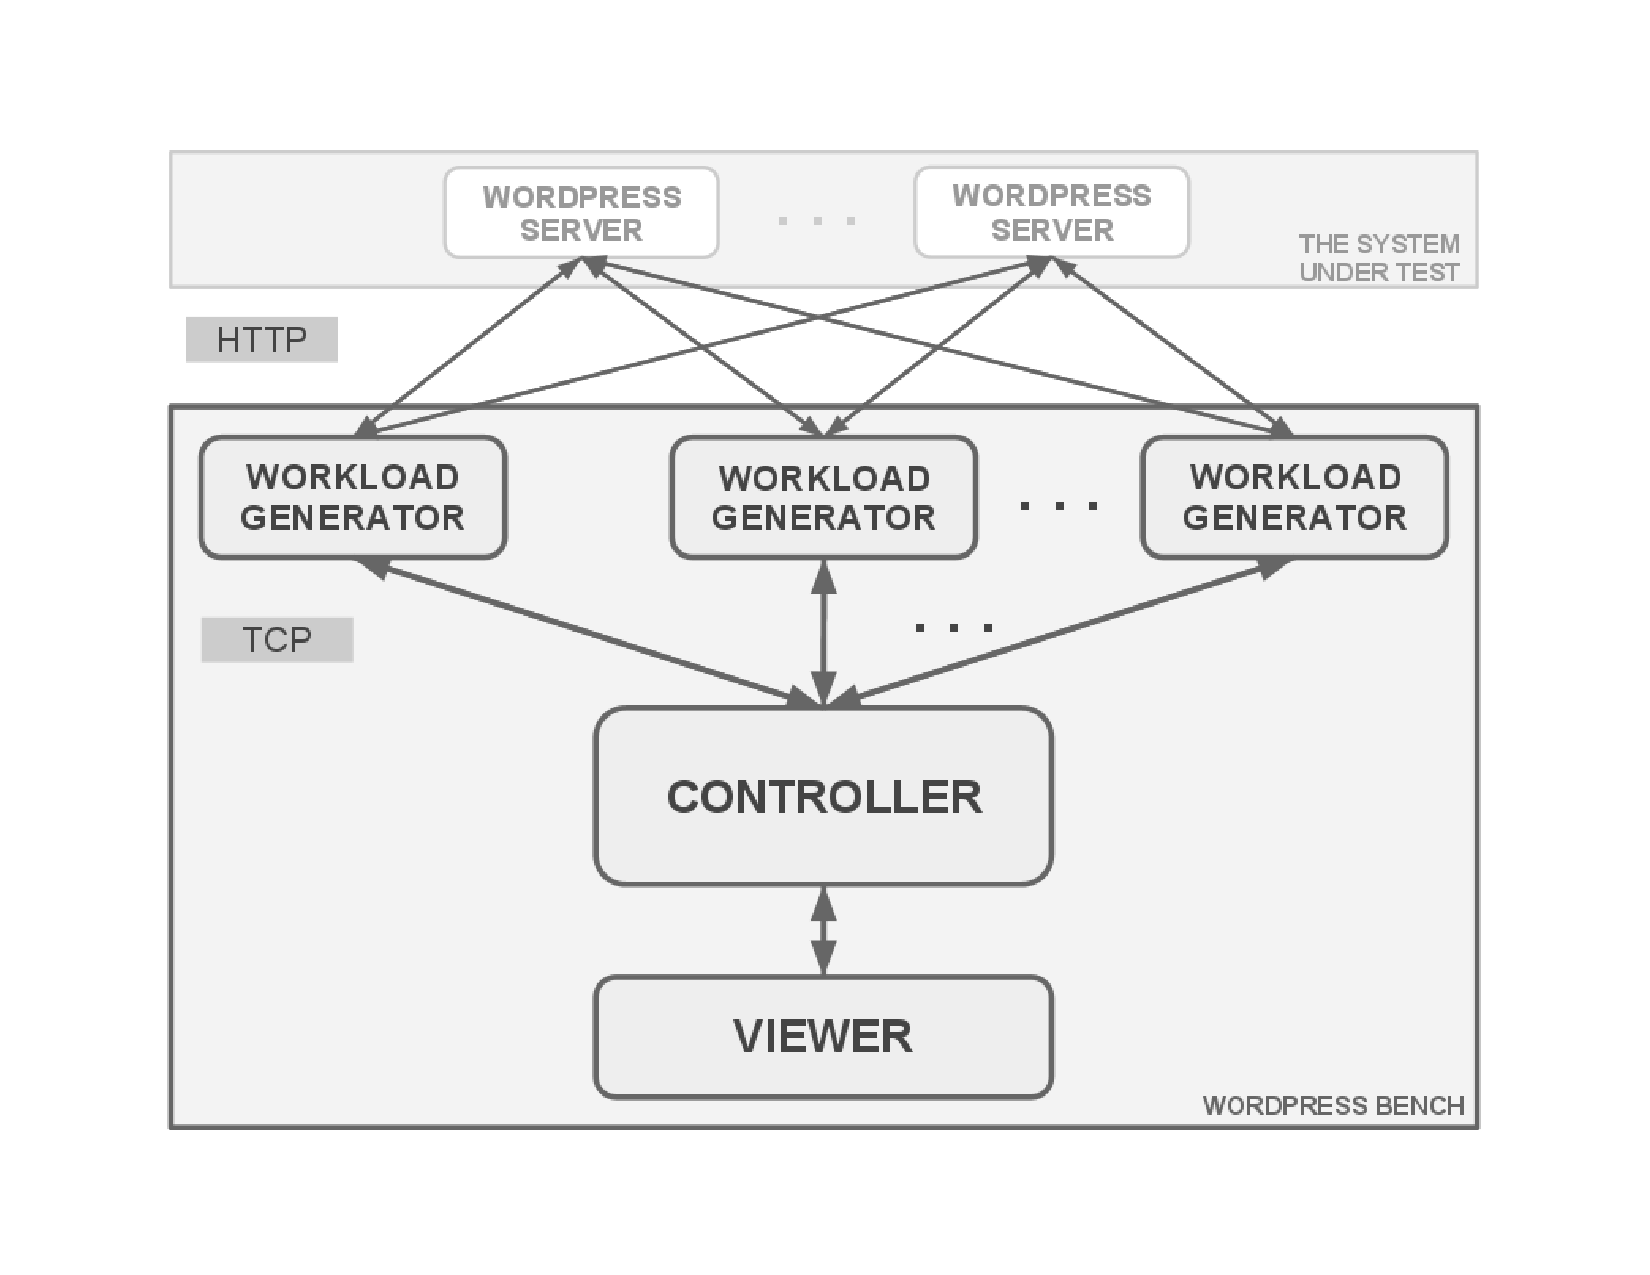
\includegraphics[trim=2.5cm 2.5cm 2.5cm 2.5cm, clip=true, scale=0.65]{src/img/WordPressBench.pdf}
    \caption{System Design}
    \end{center}
  \label{figure:system-design}
  \end{figure}

%\fig[scale=0.6]{src/img/WordPressBench.pdf}{img:system-design}{System Design}

\section{Components}
\label{sec:components}

\subsection{WordPress Web Servers}
\label{sub-sec:wordpress-web-servers}

The WordPress Web Server use Apache servers and a MySQL database. It also requires to have PHP installed on the machine. We used WordPress version 3.2 available at the development time. It allows users to read blog-posts, pages and comments. This can be done by searching by keyword, by author, by date, by category, by viewing recent posts, or simply by browsing each single blog-post. Anonymous users are allowed to post comments by providing their e-mail address. Their information remains in browser's cache through cookies, until the information is overwritten.

Additional write operations are allowed only for registered users. After logging in, they have access to extended edit functionalities, like adding comments to pages and blog-posts as registered users, or adding pages, blog-posts and blog-post categories. Users with 'Administrator' rights are allowed to create new users, or to clear the data from the database, operation performed in the initiation stage of the development.

\subsection{Workload Generator}
\label{sub-sec:workload-generator}

The Workload Generator is a component running on slaves machines. It contains a Markov matrix with all the possible states and the probabilities to make a transition to another state. 

There are three transition matrices, one for anonymous user, one for logged-out user, and another for anonymous user. This is mainly because the registered user has access to additional states and the flow of actions could be totally different from an anonymous user. The read-only user has the most restrictive operations.

The transition matrix describes the users' navigational pattern, by specifying how users navigate through the website, the functions they are allowed to use in a certain state and how often, and the frequency of transitions from one state to another. Users interact with the WordPress Website through sessions, which are sequences of consecutive requests to bring different pages from the WordPress Website. After each request, a transition is made from the current state to another state. The next state is chosen from the transition matrix which indicates for each state which are the next possible transitions. The matrix columns indicate the current state, and the matrix lines are the states which could follow. A zero in the matrix means that there is no possible transition from current state to the state indicated by the line. A non-zero value in the matrix represents the probability to make a transition to the state indicated by the line. So when choosing the next state, only a non-zero value will be chosen. For building the transition matrix we chose bigger probabilities for widely used functionalities, like reading a blog-post or posting a comment. \labelindexref{Figure}{figure:transition-table} depicts the transition table for a registered user who can log-in and perform additional write operations.

%   \begin{figure}[htb]
%     \begin{center}
%     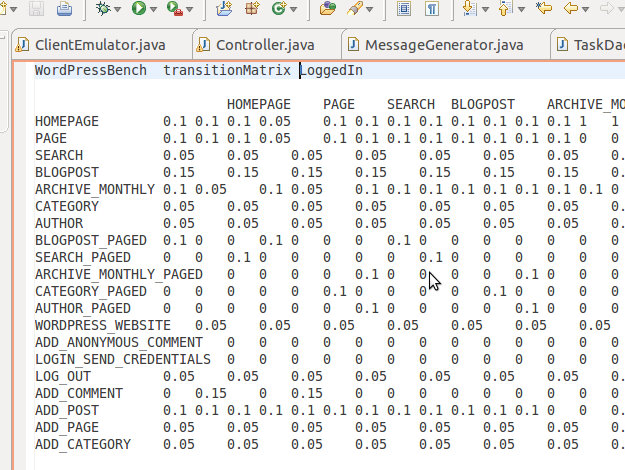
\includegraphics[scale=0.8]{src/img/transitionTable.jpg}
%     \caption{Transition matrix for a Logged-in user}
%     \end{center}
%   \end{figure}

  \begin{figure}[t]
    \centering %trim=l b r t
    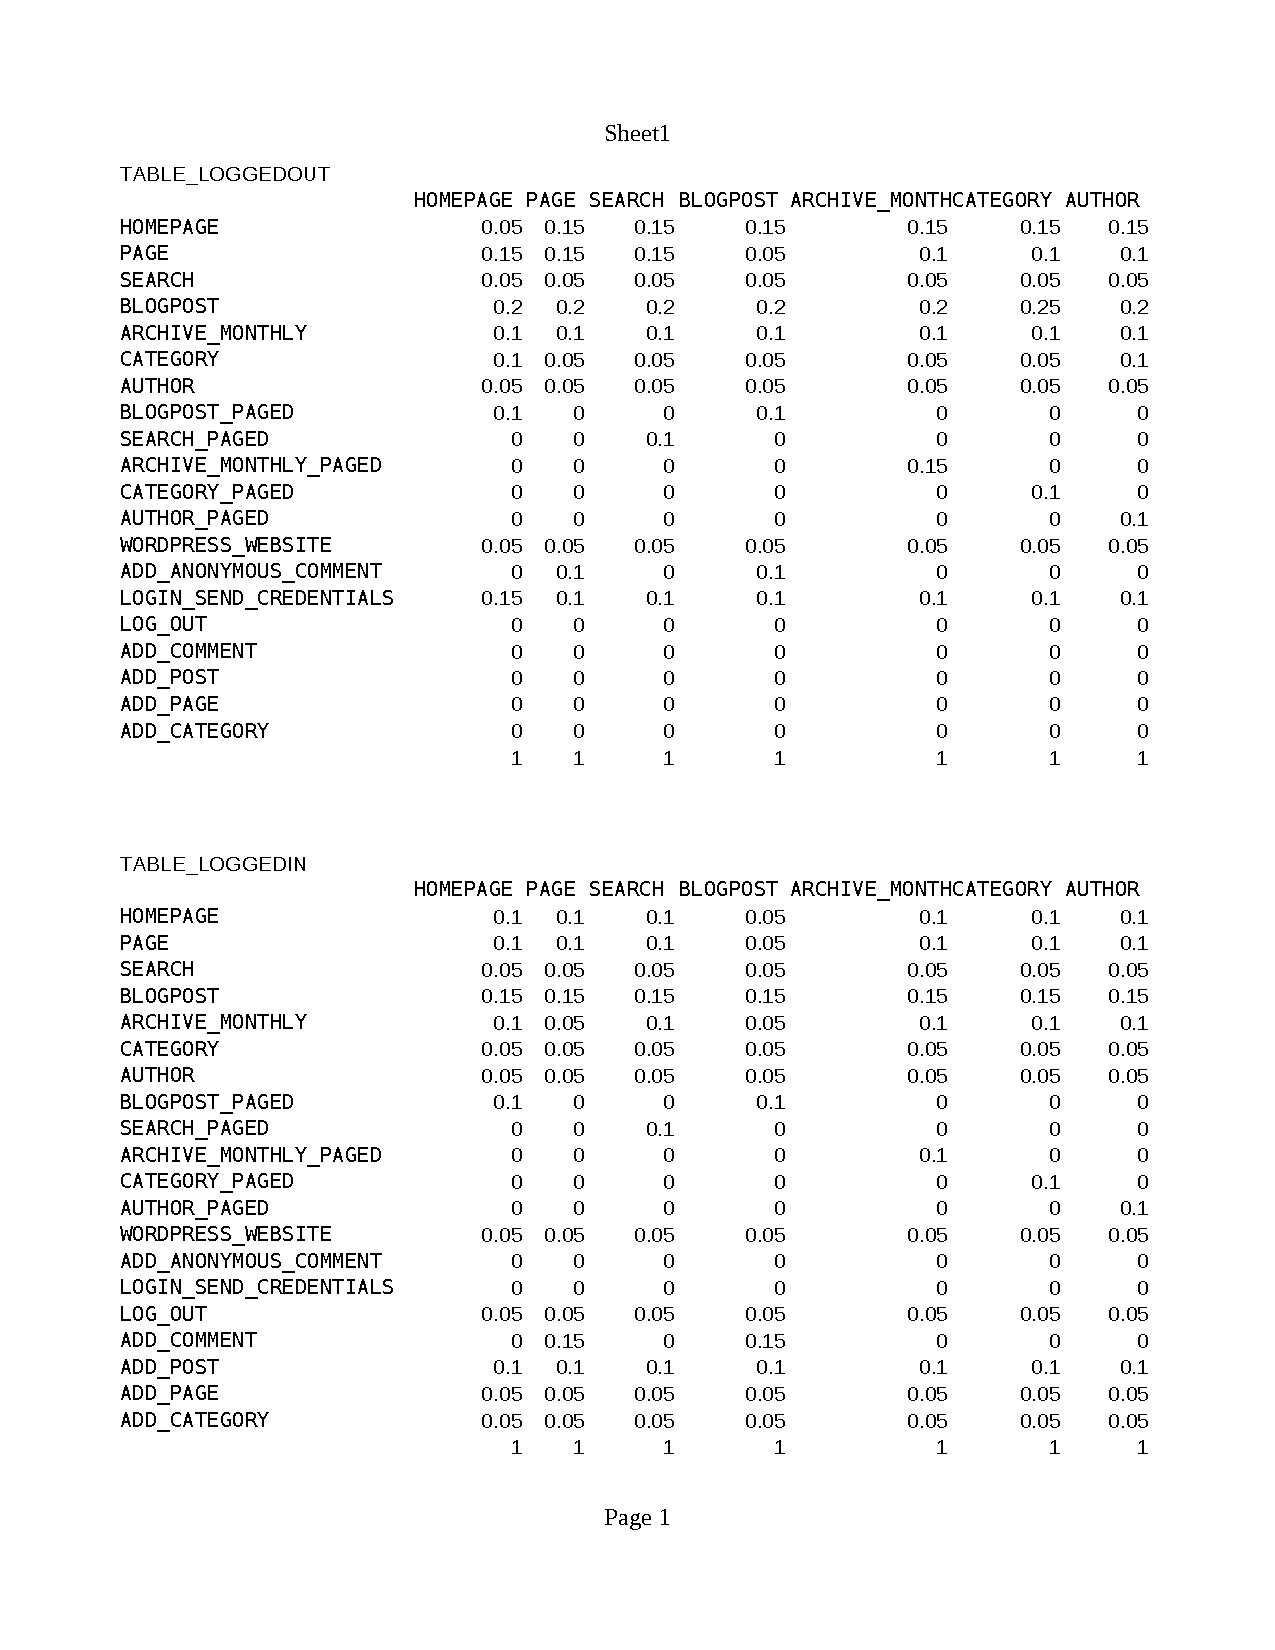
\includegraphics[trim=2cm 14cm 2cm 3.2cm, clip=true, scale=0.85]{src/img/transitionTable.pdf}
    \caption{Transition matrix for a Logged-in user}
    \label{figure:transition-table}
  \end{figure}

The HTTP requests require URLs which specify what page should be brought back. Additional information is often needed, especially for users who are logged-in, so information is either encoded in POST variables, or in cookies. The information which is requested by the WordPress servers includes user information, text for publishing, IDs, options, nonces (random number issued in previous HTML content received from WordPress server), passwords and usernames. Some of this information is generated by the Workload Generator, but the IDs or nonces are gathered from the previous HTTP page just received from the WordPress server. Cookies also need to be send back to the server, exactly as they have been received. They are used to maintain the logged-in user session, and they are reset as soon as the user logs-out. If the request is successful, and the correct page is sent back, the session makes a transition to the desired state. To simulate users more realistically and knowing that real users spend a different amount of time between requests, each emulated user has a random "think time" of at least 7 seconds between requests. For avoiding fast automated requests, WordPress rejects requests sent in a very small amount of time, so the "think time" was absolutely necessary.

In case a user logs in, the session is maintained through cookies, which need to be sent back to the Web server at each request until the user logs out. There are states which get data from HTTP POST variables, not only from GET variables encoded in URLs. In this case, the slave needs to get the keywords, IDs, from the previous page, and send it along with other random data generated on the fly, and needed by the Web server. 

While running, the Workload Generator gathers statistics about the responses time. Statistics like response time, number of errors, number of attempts before getting the response, or other such information is stored for each user along with a timestamp, and aggregated into log files which are sent to the Master at the end of the simulation.

\subsection{Controller}
\label{sub-sec:controller}

The Controller is the main command component. It has control over the Workload Generators and sends commands to them through TCP messages. The Controller can send five types of messages:
\begin{itemize}
 \item start simulation
 \item stop simulation
 \item create users
 \item add users
 \item get logfile
 \item exit
\end{itemize}

For starting the simulation, the Controller indicates the username range to be used by each Workload Generator, along with the read-write ratio. The number of users is computed afterwards for each Workload Generator. Each of them uses distinct usernames to avoid overlapping. The command for creating more users has the effect of registering a certain amount of users to the WordPress server(s). This command is generally followed by either the simulation start, or the addition of more users. The command for adding more users is send during the simulation process, when the number of user is increased, so new user sessions are initiated. The command for getting the log file simply requests the log files with statistics from each Workload Generator. This operation is usually performed after the simulation has been stopped, when data is not written anymore into the log files. Afterwards, the log files are aggregated and processed by the Controller, and data is ready to be send as input for generating graphs. The exit command stops all the components, so the Controller cannot send commands to the other machines anymore.

The log files generated by each Workload Generator output on the first column the time in seconds relative to the beginning of the simulation. This includes the initialization time. On the second column is displayed the response time for the current state, and on the third column is displayed the name of the current state. The Controller takes the log files from each Workload Generator and aggregates them by the first column, computing the average response time in one second. The third column from the initial log files is ignored.

The average response time is measured in milliseconds for a finer granularity, and the relative time is measured in seconds. We chose to have the relative time from the beginning of the simulation and not the real time. This decision was made in order to avoid the case when the machines are not synchronized, so the local time for each measurement would be different.

The Workload Generators compute additional statistics, and at the end of the log files are displayed additional statistics for each state. The percent, the number of transitions, number of errors, the minimum time, the maximum time, and the average time are computed for each transitioned state. The overall average time for the current Workload Generator is computed and displayed at the end of the log file.

\section{Component Connections}
\label{sec:component-connections}

Data flow between components is sent through two types of protocols: HTTP and TCP. HTTP protocol is used for sending GET methods with cookies and POST data to the WordPress Web server. HTTP messages are sent back in response with the requested pages, or error codes if necessary. 

TCP protocol is used to send commands from the Controller to the Workload Generators. The Controller's commands have designated code values, so a number from 0 to 5 encodes one of the six possible commands listed above. This code could be followed by two numbers representing the user id range to be used by the current worker. A third number represented by a double value indicates the read-only percent of the requests. After each command an acknowledgement message is sent to the Controller to confirm that the message has been received and the requested operation was executed. In the case of the "Get log" command, the log files are sent through the same TCP connection and written to local log files on the Controller machine. 

\section{Workflow}
\label{sec:workflow}

After the benchmark simulation is started, the first step is to delete all the data from WordPress server's database. This is performed by a single thread with "Administrator" rights on a Workload Generator. Afterwards the Controller sends command to a Workload Generator to create a number of users. This operation will be performed similarly to previous data deletion step. 

For starting the simulation each Workload Generator receives a user ID range. Their count represents the number of emulated users, so this is the number of threads which will be created. Each thread emulates a user and sends HTTP requests to the WordPress Web server placed on the system under test. The states are chosen randomly from one of the transition matrix (read-only matrix, logged-in matrix, or logged-out matrix) and for each request the response time is logged along with the current time and state name. 

The Controller can send other additional messages to the Workload Generators, like adding more users. In this case an additional message will be sent in order to create more users, so a thread on a single Workload Generator will create the additional number of users if necessary. Afterwards each machine will add the corresponding users by creating more threads which emulate users, using the newly created user IDs. 

When the Controller requests the end of the simulation, each thread from the Workload Generators will resume, but the machine will continue to receive new commands, the most common one being "Get logfile". In this case the log files are sent through TCP connection and aggregated on the Controller. The exit command sent by the Controller is the one which completely stops all the components. The simulation yields a number of log files which are ready to be processed.

\section{Tools and Technologies}
\label{sec:tools-and-technologies}

As mentioned before, we decided to use an existent Web server platform. We used WordPress because it is a very mature and reliable platform. Is is widely used by millions of users and therefore it went through extensive testing and constant updates. WordPress requires an Apache server for running the Web server. It listens HTTP requests coming from the Workload Generators. 

WordPress is using a MySQL database as well, where it stores the data displayed on its website: user credentials, user settings, and Web blog content like blogposts, comments, pages, categories and details about each of them. WordPress as a predefined schema of tables which is created at each setup. The benchmark interacts directly with the MySQL database by using commands to delete the data at the beginning of each simulation.

The system is implemented entirely in Java. We made this choice because it offers ease of development, a good API and offers good support for TCP and HTTP protocols usage. We used Java sockets and performed GET requests to the Web servers on the system under test.
